\documentclass[12pt,a5paper]{article}
\usepackage[margin=.5cm]{geometry}
\usepackage[utf8]{inputenc}
\usepackage[IL2]{fontenc}
\usepackage[czech]{babel}
\usepackage{microtype}
\usepackage{amssymb}
\usepackage{amsthm}
\usepackage{amsmath}
\usepackage{xcolor}
\usepackage{graphicx}

\usepackage[inline]{enumitem}

\newcommand{\hint}[1]{{\color{gray}\footnotesize\noindent(Nápověda: #1)}}

\setlist[enumerate]{label={(\alph*)},topsep=\smallskipamount,itemsep=\smallskipamount,parsep=0pt,itemjoin={\quad}}
\setlist[itemize]{topsep=\smallskipamount,noitemsep}

\def\tisk{%
\newbox\shipouthackbox
\pdfpagewidth=2\pdfpagewidth
\let\oldshipout=\shipout
\def\shipout{\afterassignment\zdvojtmp \setbox\shipouthackbox=}%
\def\zdvojtmp{\aftergroup\zdvoj}%
\def\zdvoj{%
    \oldshipout\vbox{\hbox{%
        \copy\shipouthackbox
        \hskip\dimexpr .5\pdfpagewidth-\wd\shipouthackbox\relax
        \box\shipouthackbox
    }}%
}}%



\newtheorem*{poz}{Pozorování}

\theoremstyle{definition}
\newtheorem{uloha}{Úloha}
\newtheorem{suloha}[uloha]{\llap{$\star$ }Úloha}
\newtheorem*{bonus}{Bonus}
\newtheorem*{defn}{Definice}

\pagestyle{empty}

\let\ee\expandafter

\def\vysld{}
\let\printvysl\relax
\let\printalphvysl\relax

\makeatletter
\def\vyslplain#1{\ee\ee\ee\gdef\ee\ee\ee\vysld\ee\ee\ee{\ee\vysld\ee\printvysl\ee{\the\c@uloha}{#1}}}
\let\vysl\vyslplain

\def\locvysl#1{\ee\gdef\ee\locvysld\ee{\locvysld\item #1}}
\let\lv\locvysl

\newenvironment{ulohav}[1][]{\begin{uloha}[#1]\gdef\locvysld{\begin{enumerate*}}}{\ee\vyslplain\ee{\locvysld\end{enumerate*}}\end{uloha}}
\newenvironment{sulohav}[1][]{\begin{suloha}[#1]\gdef\locvysld{\begin{enumerate*}}}{\ee\vyslplain\ee{\locvysld\end{enumerate*}}\end{suloha}}

\makeatother

\begin{document}

% \tisk

\section*{Eulerovské grafy}

\begin{uloha}
Nakreslete jedním tahem následující grafy:
% obrazky z Matouska-Nesetrila
\[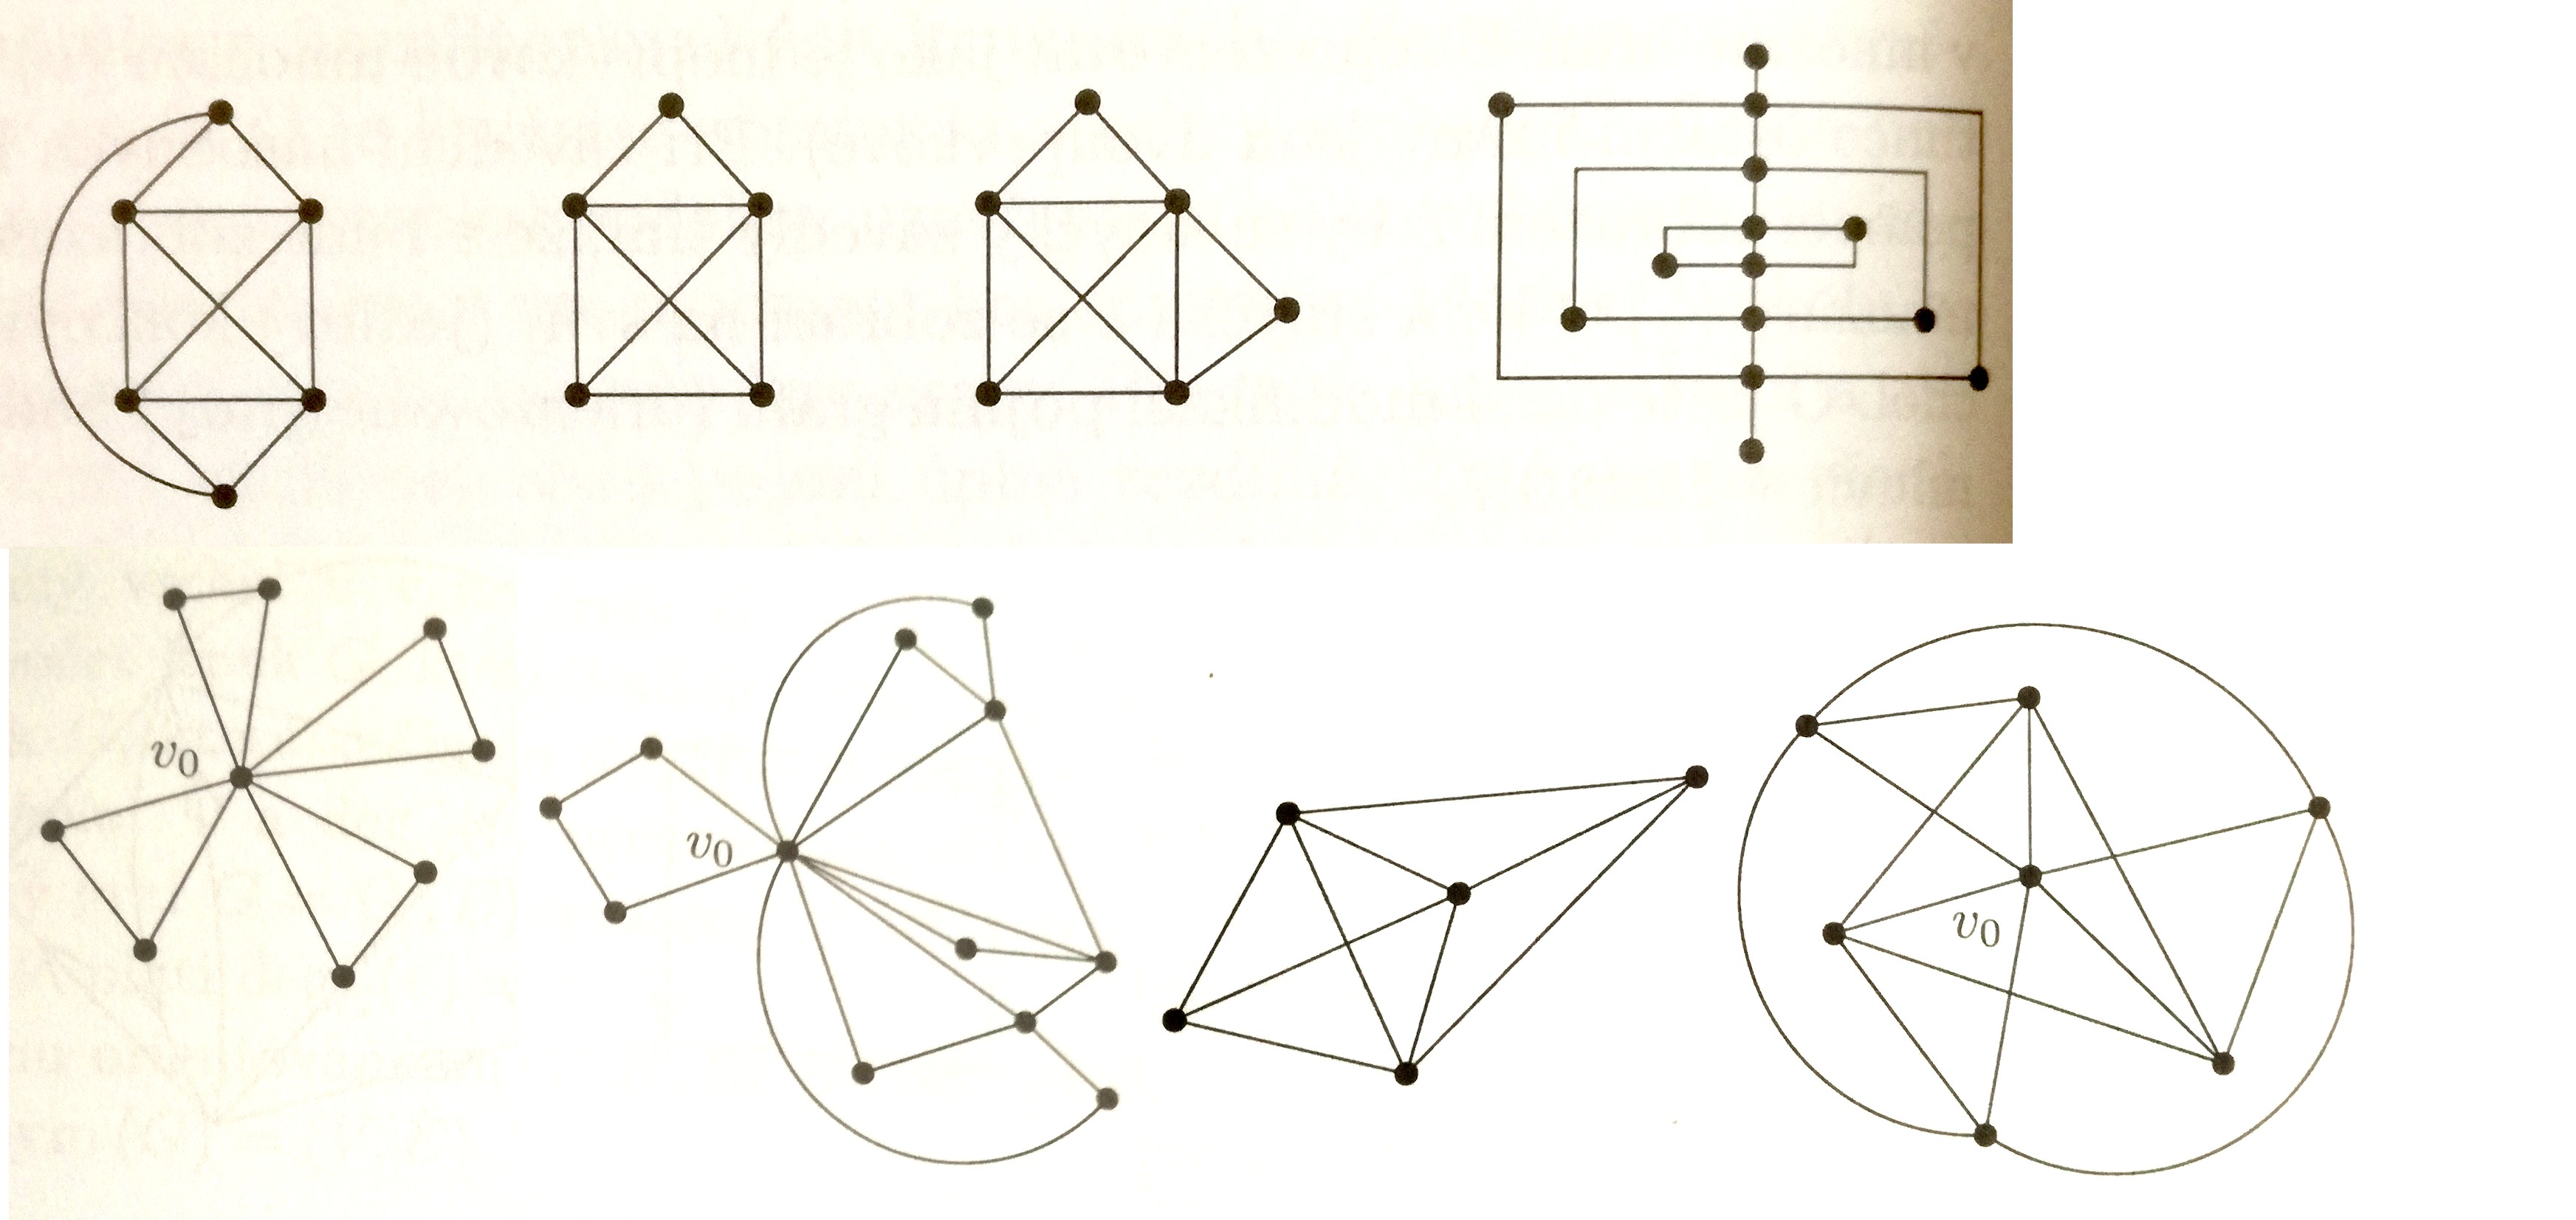
\includegraphics[width=.9\hsize]{euler.jpg}\]
\end{uloha}

\begin{uloha}
Najděte příklady grafů, které nelze nakreslit jedním tahem. Zkuste vyslovit hypotézu, jak se na grafu pozná, zda to vyjde. (Pokud nevíte, tak vám dám nápovědu). Rozmyslete si, že taková podmínka musí být splněna.
\end{uloha}

\begin{uloha}
Které z grafů z druhého řádku první úlohy nakreslíme jedním tahem, i když budeme kreslit \uv{úplně náhodně} začínajíce ve $v_0$?
\end{uloha}

\begin{uloha}
Jak by se situace změnila, kdyby hrany byly \emph{orientované}, tj. šipky?
\[ 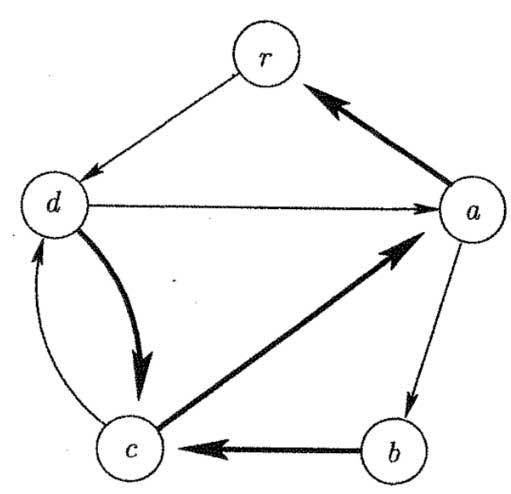
\includegraphics[width=3cm]{orient_1.jpg}\qquad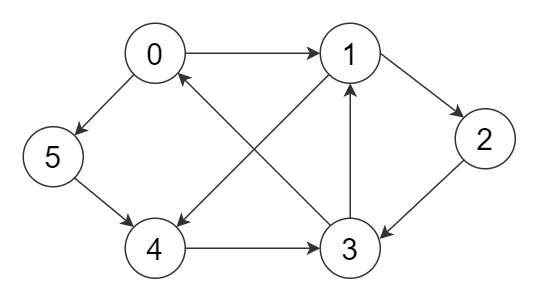
\includegraphics[width=5cm]{orient_2.png} \]
\end{uloha}

\begin{uloha}
Napište 16 jedniček/nul \uv{dokola} tak, aby se ve výsledné posloupnosti nacházelo každé z čísel 0--15 zapsané ve dvojkové soustavě (správným směrem). Např. 00011101 (se \uv{slepenými konci}) to je pro 0--7.
\end{uloha}


\end{document}